\section{Results}

\subsection{Linear VS não-linear}
\begin{frame}
  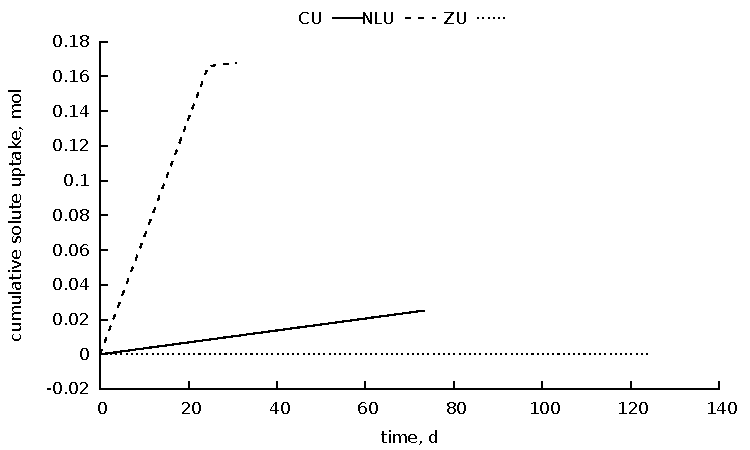
\includegraphics[height=3.cm]{accumxt.pdf}
  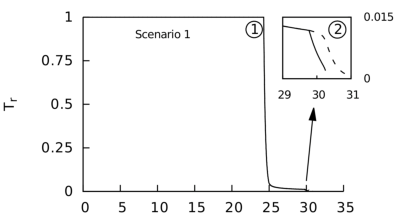
\includegraphics[height=3.cm]{diff_tr1.pdf}\\[.5cm]
  
  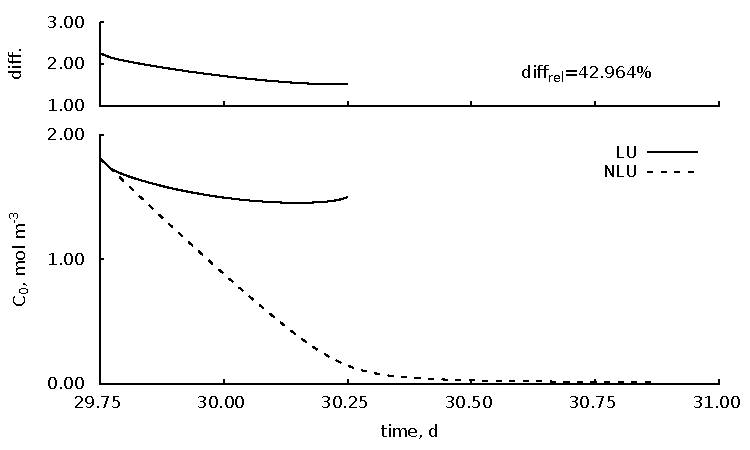
\includegraphics[height=3.3cm]{diffs_t.pdf}
  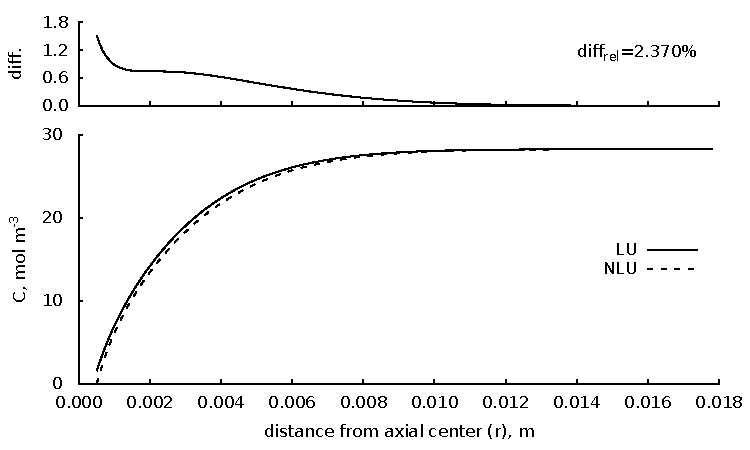
\includegraphics[height=3.3cm]{diffs_r.pdf}

  Diferenças significativas somente em $C_0(t)$ $\rightarrow$ NLU é preferido $\rightarrow$ instabilidade, menores $\Delta t$\\
  LU $\rightarrow$ preferido quando se deseja usar $Ac(t)$ ou $C(r)$ $\rightarrow$ maiores $\Delta t$ (estável)
\end{frame}

\subsection{Comparação dos modelos}
\begin{frame}
  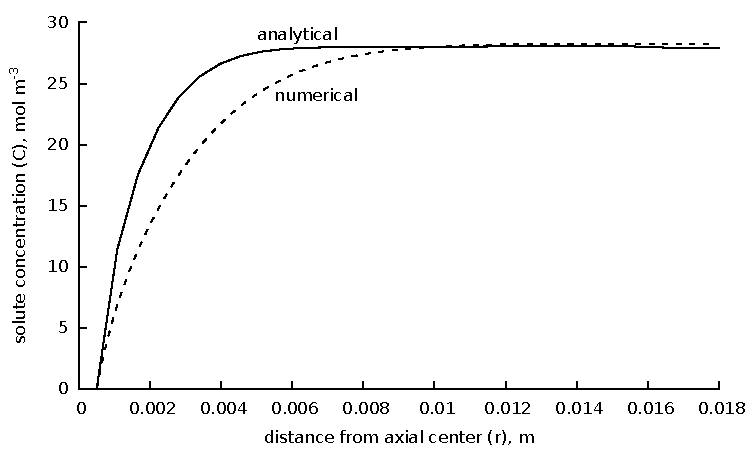
\includegraphics[height=3.3cm]{analytic_cushman.pdf}
  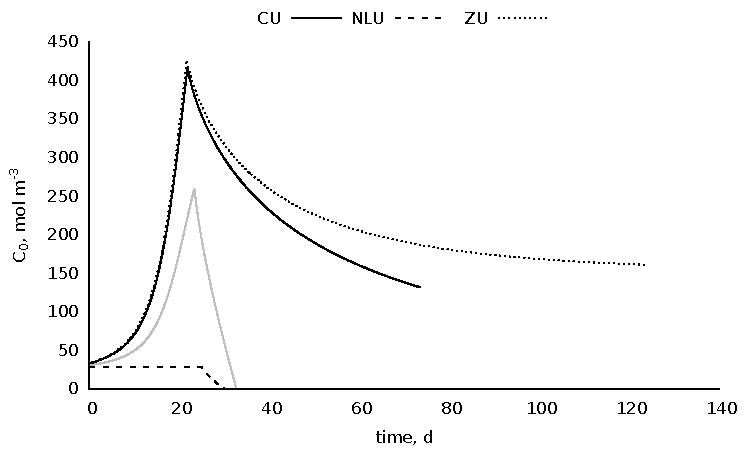
\includegraphics[height=3.3cm]{cxt_comp.pdf}\\[.5cm]
  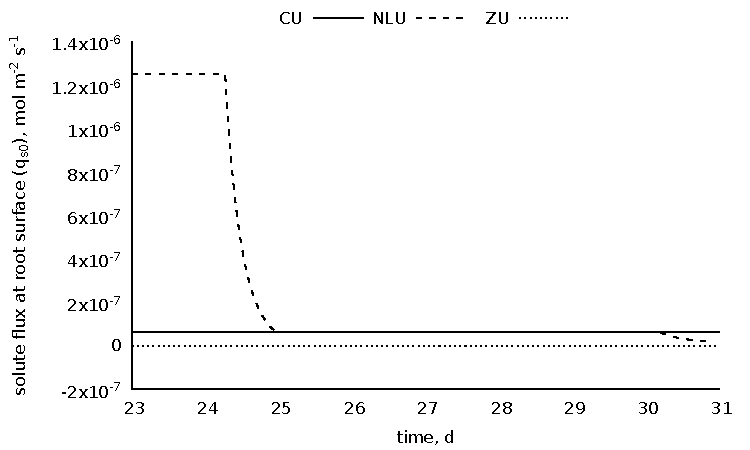
\includegraphics[height=3.3cm]{qsxt1_detail.pdf}
  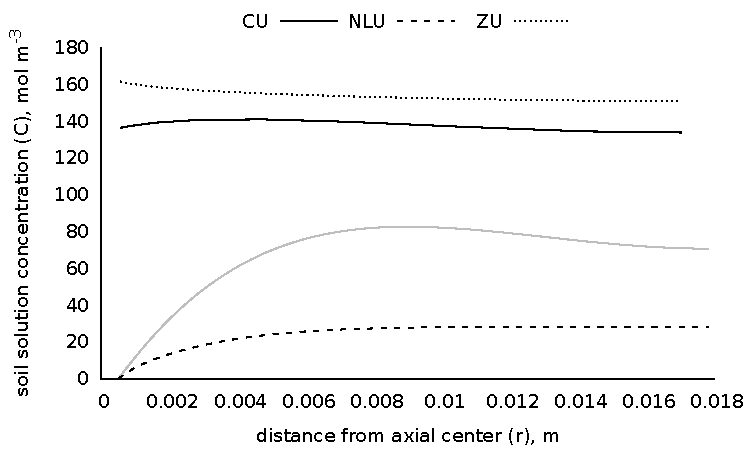
\includegraphics[height=3.3cm]{cxr_comp.pdf}

  Concentração de soluto dentro da planta não é considerada $\rightarrow$ elevada extração em altas concentrações
\end{frame}

\subsection{Resultados do modelo (NLU)}
\begin{frame}
  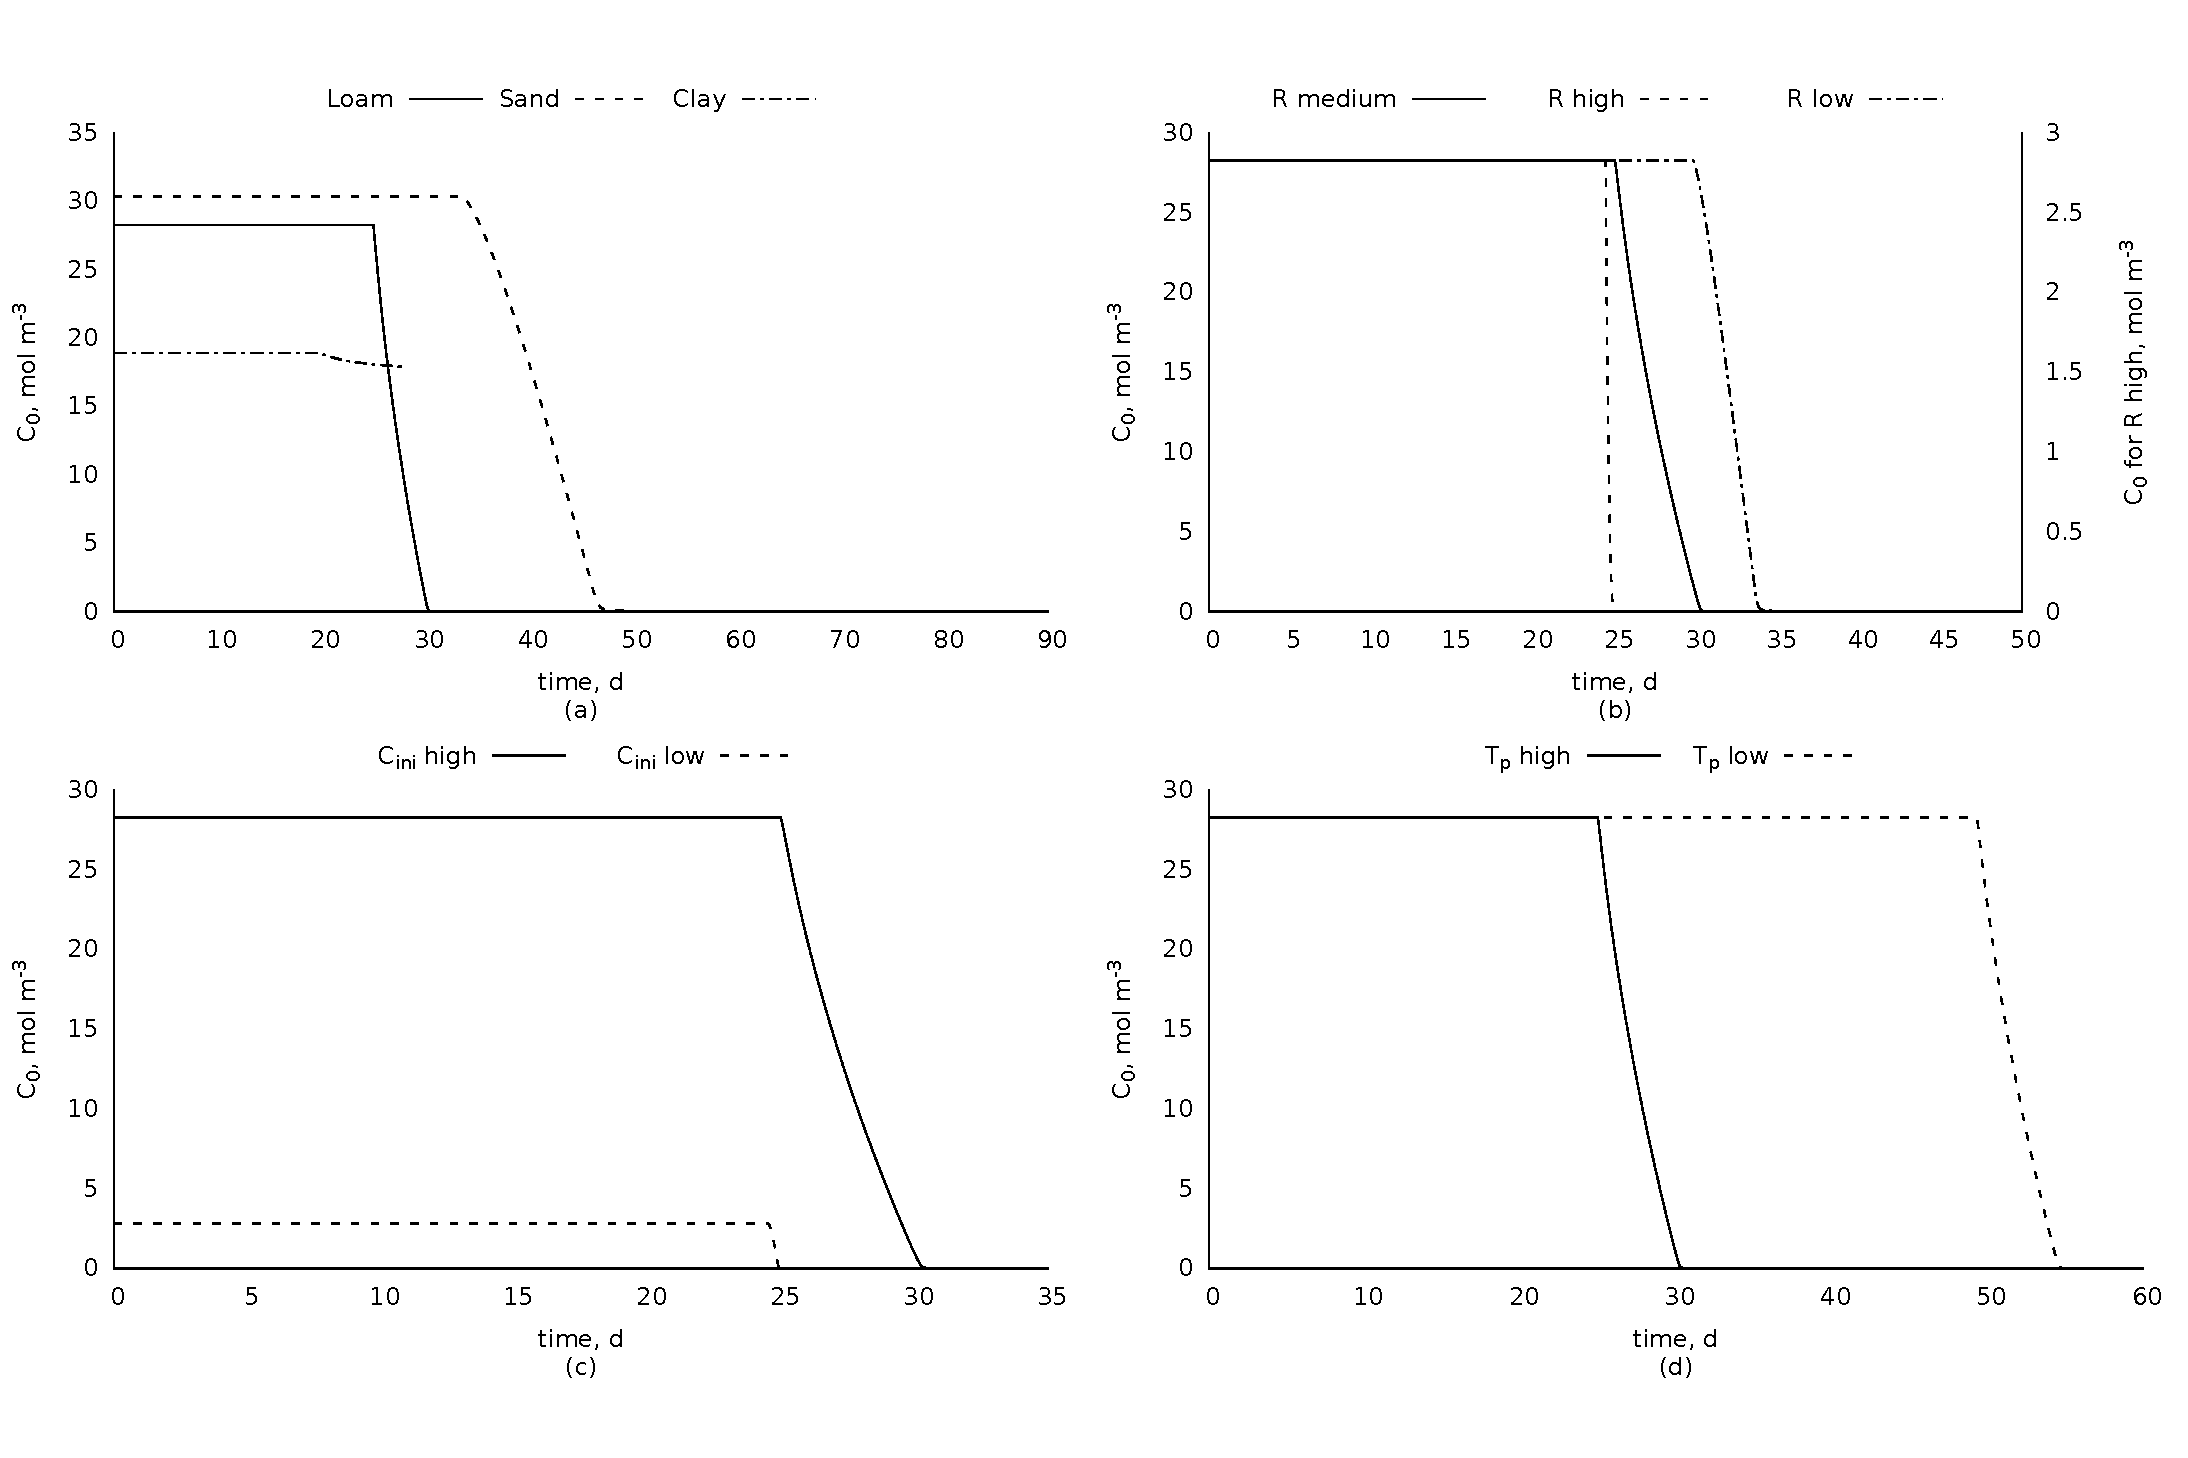
\includegraphics[height=7.3cm]{C_t.pdf}
\end{frame}
\begin{frame}
  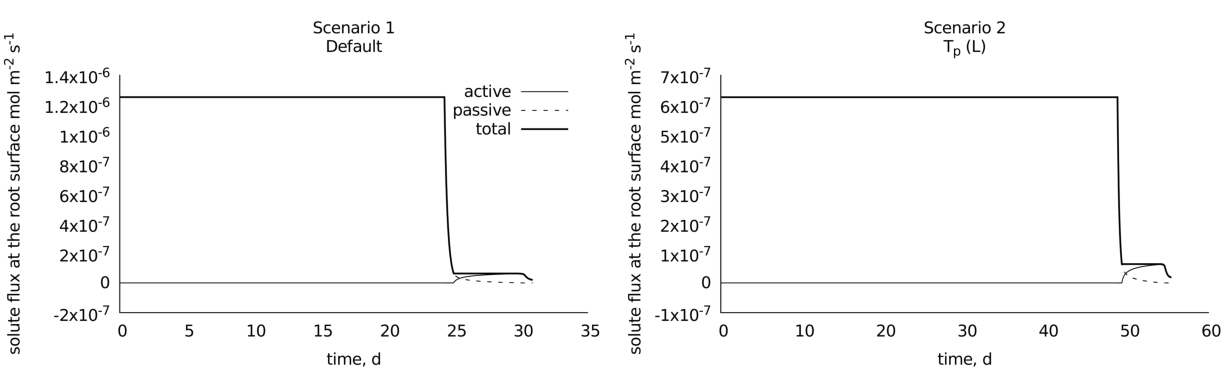
\includegraphics[height=3.3cm]{contribxt1e2.pdf}\\[.5cm]
  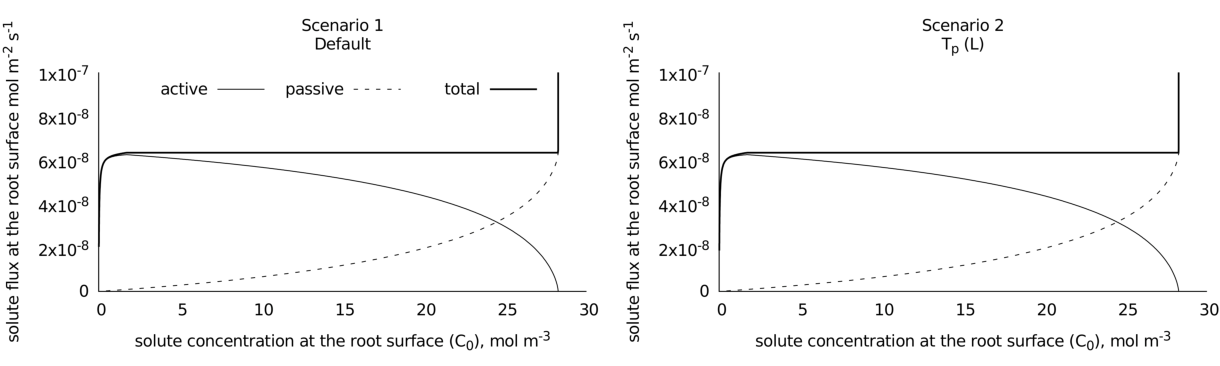
\includegraphics[height=3.3cm]{contribxc1e2.pdf}
\end{frame}
\begin{frame}
  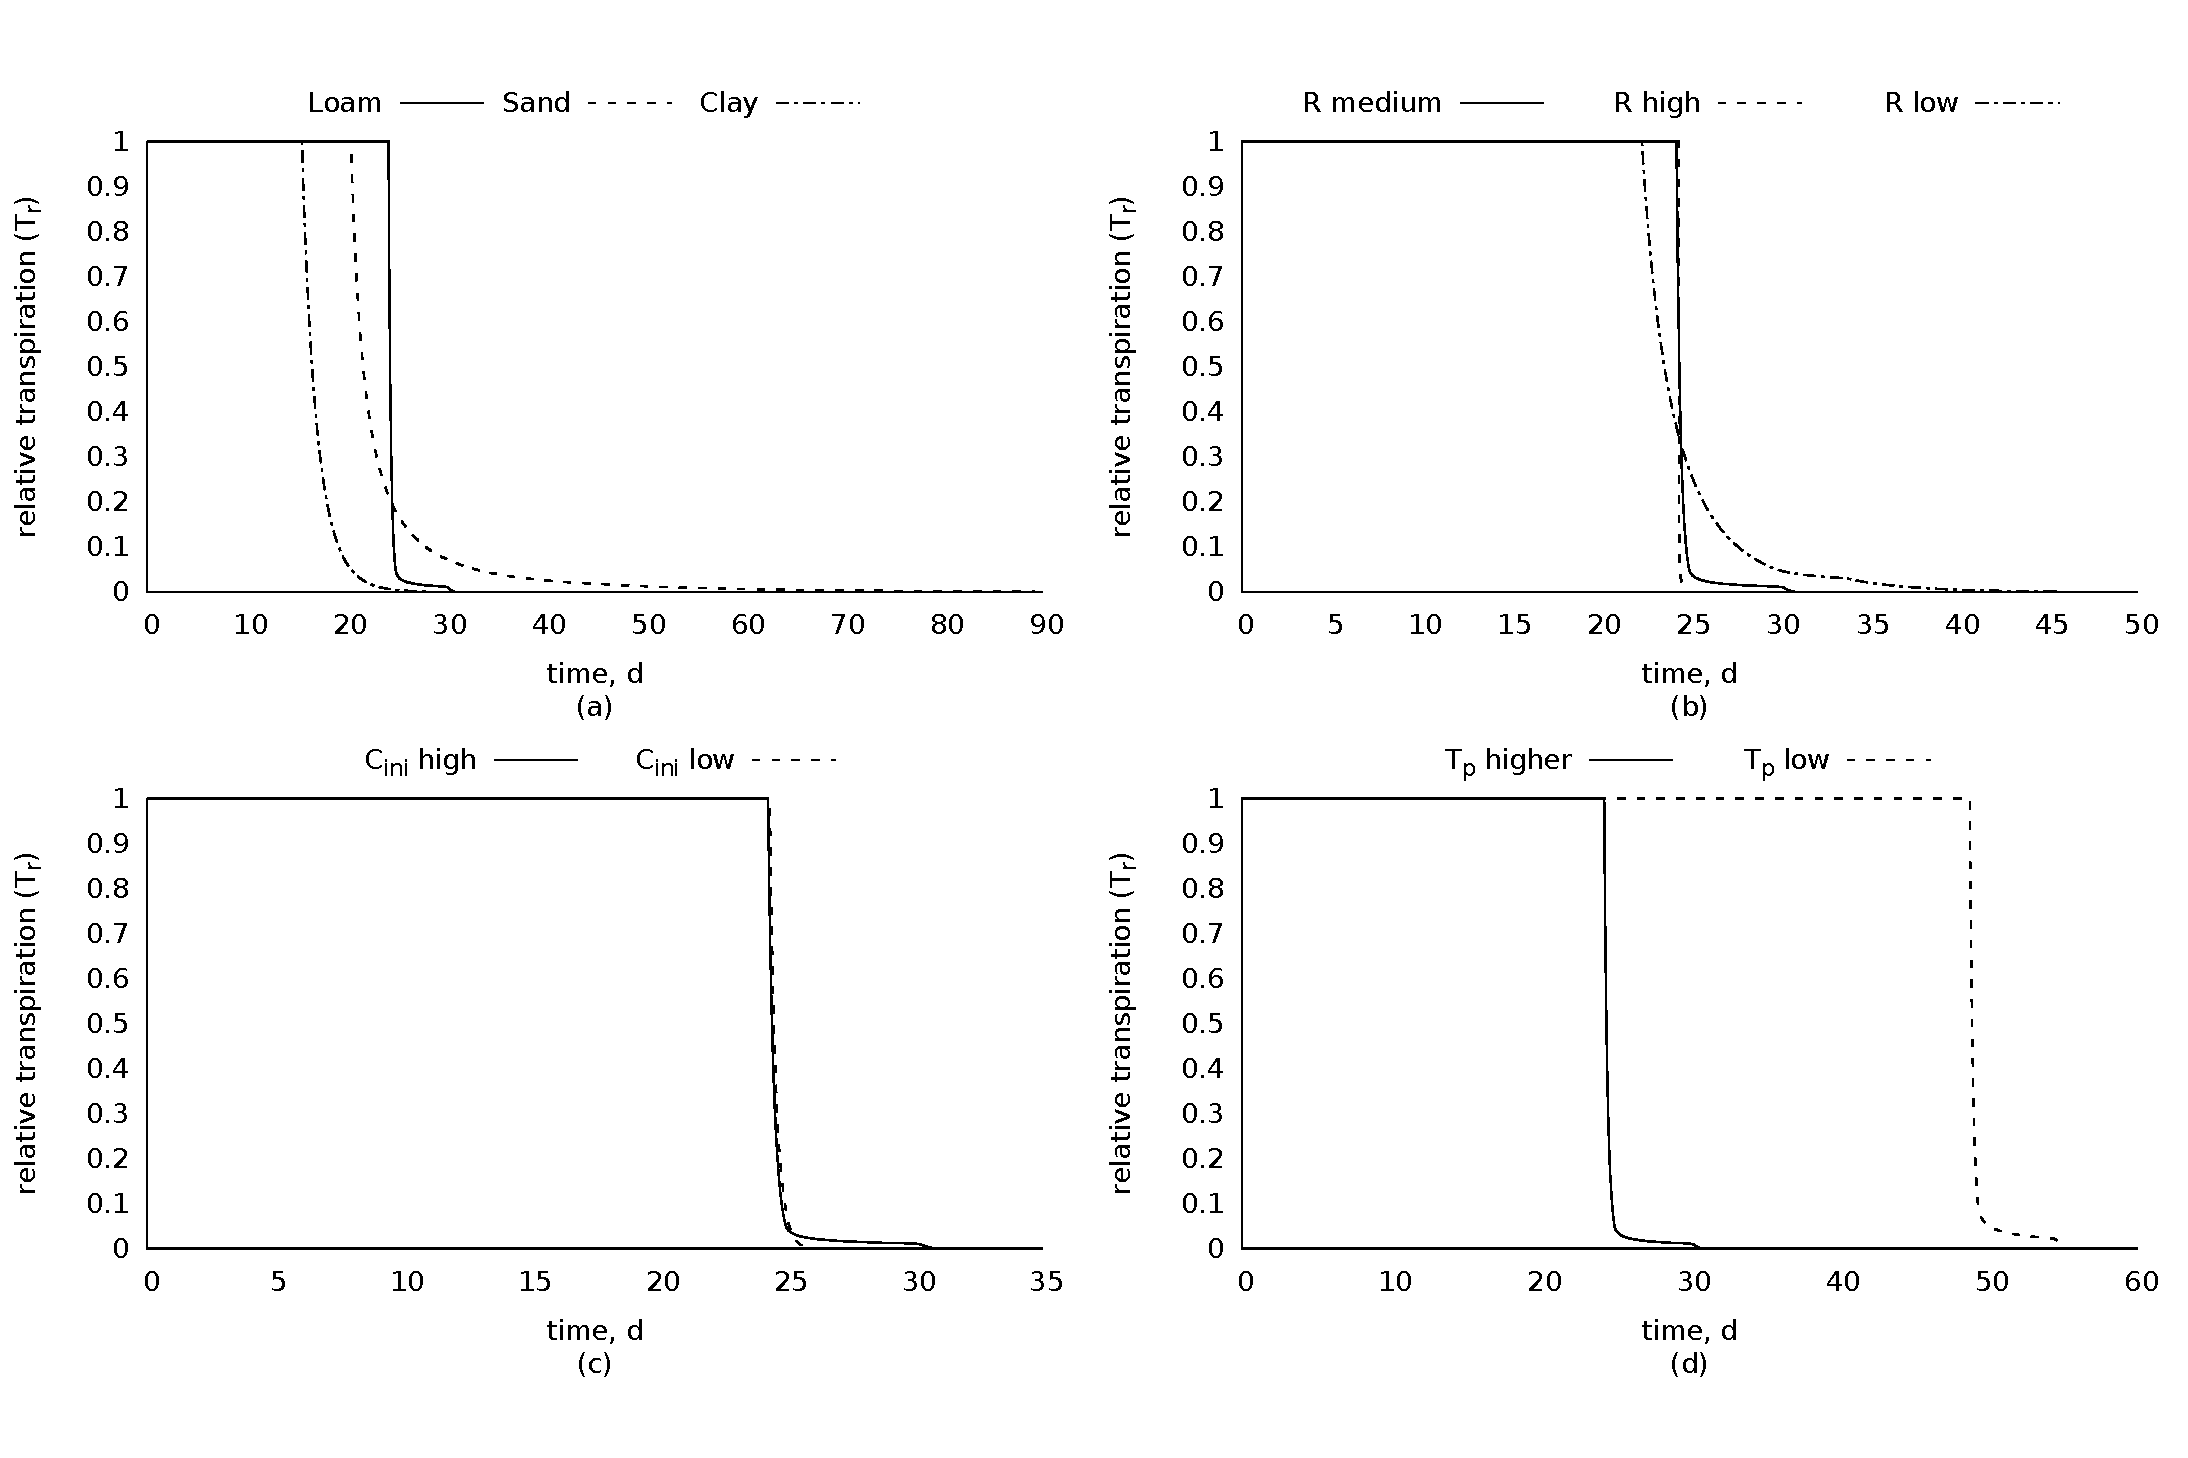
\includegraphics[height=7.3cm]{Tr_t.pdf}
\end{frame}

\subsection{Análise de sensibilidade}
\begin{frame}
  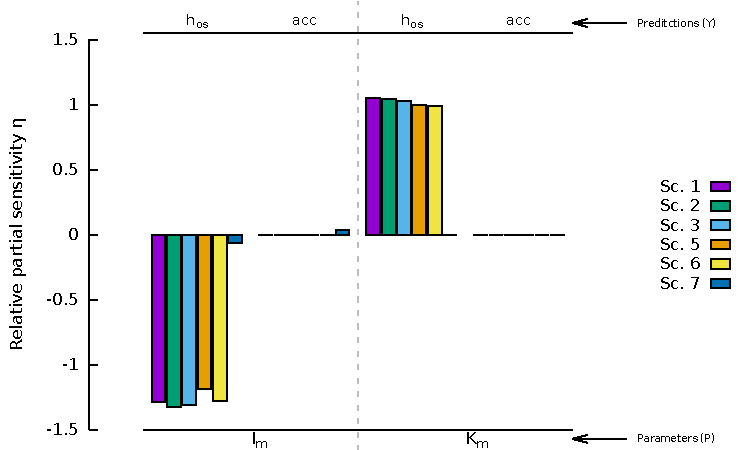
\includegraphics[height=3.3cm]{final_everybar_MM_rest.pdf}
  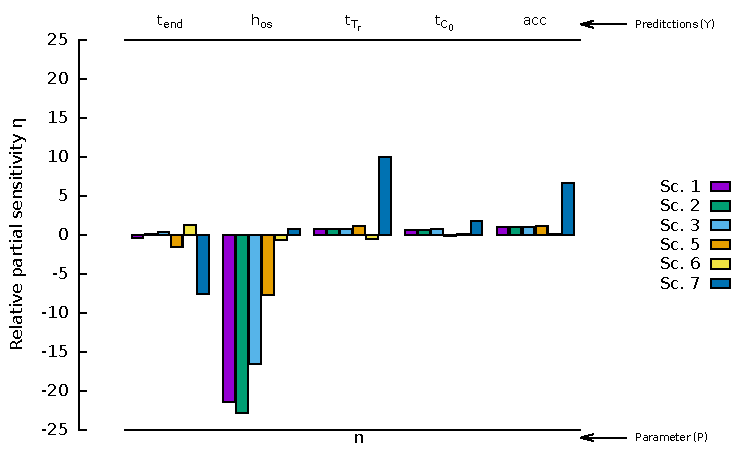
\includegraphics[height=3.3cm]{final_large.pdf}\\[.5cm]
  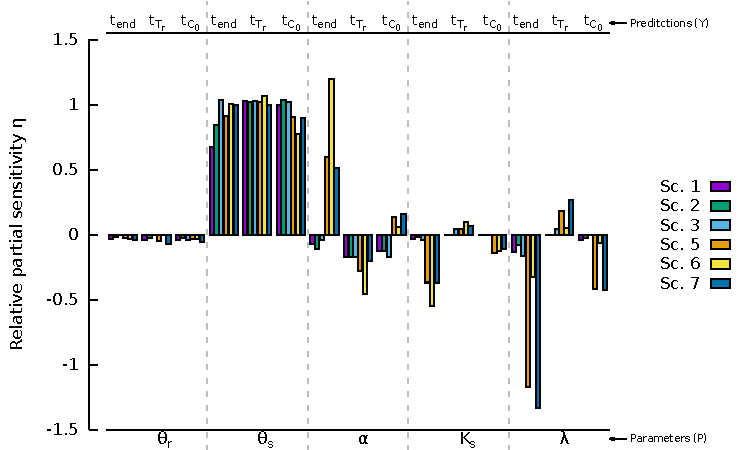
\includegraphics[height=3.3cm]{final_every_bar_soil_time.pdf}
  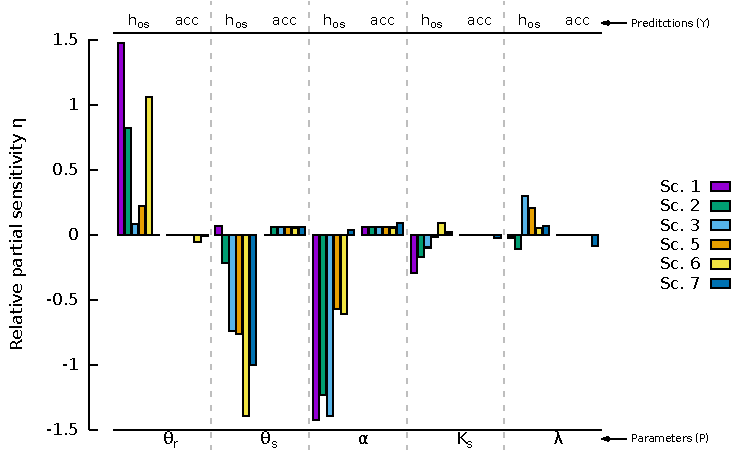
\includegraphics[height=3.3cm]{final_every_bar_soil_rest.pdf}


\end{frame}
